\documentclass[slovene,11pt,a4paper]{article}
%\usepackage{fullpage}
\usepackage[margin=2cm]{geometry}

\usepackage[T1]{fontenc}



%dodatni paketki:
\usepackage{braket} %paket za bra in ket
\usepackage{graphicx}
\usepackage{amsmath,amsfonts,amsthm} %matematicni paket
\usepackage{color} % omogoča barvno pisanje
\usepackage[utf8]
{inputenc}
\usepackage[slovene]{babel} % slovenski jezik/hyphenation
\usepackage{hyperref} %naredi vse povezave rečerenc, kazala,...
\numberwithin{equation}{section} % Number equations within sections (i.e. 1.1, 1.2, 2.1, 2.2 instead of 1, 2, 3, 4)
\numberwithin{figure}{section} % Number figures within sections (i.e. 1.1, 1.2, 2.1, 2.2 instead of 1, 2, 3, 4)
\numberwithin{table}{section} % Number tables within sections (i.e. 1.1, 1.2, 2.1, 2.2 instead of 1, 2, 3, 4)
\usepackage{eurosym} %za znak €

\usepackage{mathrsfs}
\usepackage{mathabx} % za kemisjke smeri in naslednje 3 vstrice
\catcode`_=12
\begingroup\lccode`~=`_\lowercase{\endgroup\let~\sb}
\mathcode`_="8000


\usepackage{placeins}

\usepackage[margin=2cm]{geometry}



\begin{document}
\begin{titlepage}

\newcommand{\HRule}{\rule{\linewidth}{0.5mm}} % Defines a new command for the horizontal lines, change thickness here

\center % Center everything on the page

%----------------------------------------------------------------------------------------
%	LOGO
%----------------------------------------------------------------------------------------

%\includegraphics{Logo}\\[1cm] % Include a department/university logo - this will require the graphicx package
 
%----------------------------------------------------------------------------------------


\includegraphics[width=2cm]{slike/aaa}\\[0.5cm]
 
%----------------------------------------------------------------------------------------
%	NASLOV DELA
%----------------------------------------------------------------------------------------
\textit{Univerza v Ljubljani}\\
\textit{Fakulteta za {\color{red}matematiko in fiziko}}\\[0.5cm]

\emph{Oddelek za fiziko}\\[0.5cm] % Oddelek za fiziko


%----------------------------------------------------------------------------------------
%	TITLE SECTION
%--------------------------------------------------------------------------------------
\HRule \\[0.4cm]
\huge {\bfseries 13. naloga: - Metoda maksimalne entropije}\\[0.4cm] % NASLOV SEMINARJA
\HRule \\[0.5cm] 

 \textsc{\large Poročilo pri predmetu modelska analiza 1}\\
 \textsc{\large 2015/2016}\\[1cm] % SEMINASKO DELO
 
%----------------------------------------------------------------------------------------
%	AUTHOR SECTION
%----------------------------------------------------------------------------------------



% If you don't want a supervisor, uncomment the two lines below and remove the section above
\Large \emph{Avtor:}\\
Klemen \textsc{Rahne}\\
28152028\\[2cm]
%----------------------------------------------------------------------------------------
%	DATUM
%----------------------------------------------------------------------------------------

{\large \today } \\[0.5cm] % Date, change the \today to a set date if you want to be precise

	

\end{titlepage}


%----------------------------------------------------------------------------------------
%	KAZALO
%----------------------------------------------------------------------------------------

%\tableofcontents

%----------------------------------------------------------------------------------------
%	ZAČETEK TEKSTA
%----------------------------------------------------------------------------------------


\section{Frekvenčni spekter}
V tej nalogi si bomo pogledali metodo maksimalne entropije. V tej metodi trenutni signal zapišemo kot vsota predhodnih signalov pomnoženimi s primernimi koeficienti:
\begin{equation}
y_i=\sum_{k=1}^{N} a_k y_{i-k}
\end{equation}

Moč takega signala se v frekvenčni obliki zapiše kot:
\begin{equation}
P(f)=|S(f)|^2=\frac{a_0^2}{|1+\sum_{k=1}^N a_k e^{i 2 \pi k f}|^2}
\end{equation}
Frekvenca $f$ je diskretna in je v enotah frekvenci vzorčenja $f_S=\frac{1}{N}$, kjer je $N$ število točk. Zaradi Nyqusitovega kriterija je frekvenca omejena na $\frac{1}{2}$ vzorčne frekvence. Oglejmo si najprej na preprostem signalu, ki bo vsota dveh sinusnih signalov:
\begin{equation}
\label{eq-signal1}
y_k= \sin(75 x_k) + \sin( 85 x_k) \quad x_k= k \frac{2 \pi}{N}
\end{equation}
Signalu smo priredili $512$ točk oz. v diskretnem imamo sedaj frekvenci $0.146$ za $\sin(75x)$ in $0.166$ za $\sin(85x)$.


\begin{figure}[!htb]
\centering
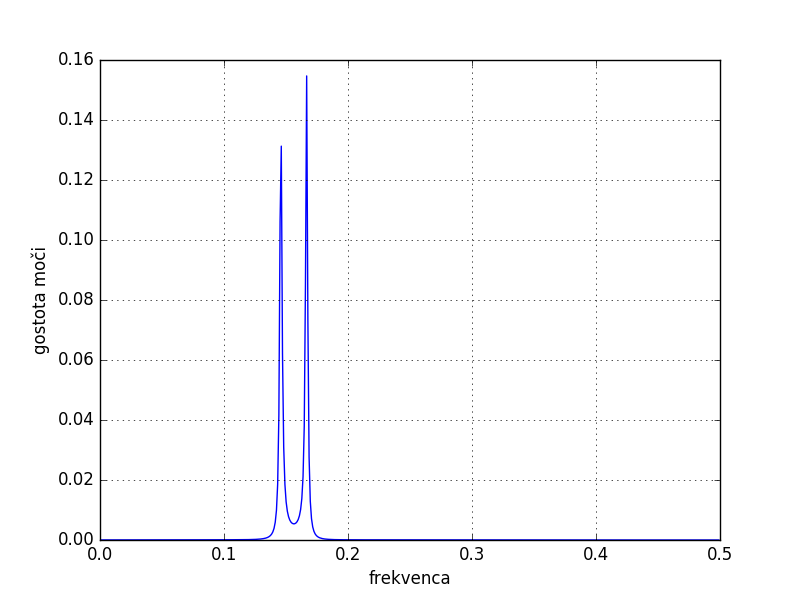
\includegraphics[scale=0.5]{slike/sin_2_frekvenci_osnovno.png}
%\caption{second figure}
\caption{Frekvenčna slika signala \ref{eq-signal1}. Opazimo da ima dva izrazita vrha, vendar njuni amplitudi nista enaki. Uporabljeno je bilo $20$ koeficientov.}
\end{figure}

V zgornjem primeru smo za prikaz uporabili dve točno določeni frekvenci in znano število koeficientov. Predpostavimo, da sta ločljivost frekvence odvisna od števila vzorčnih točk in števila koeficientov (to trditev bomo pogledali v primerih v naslednjem poglavju). Poglejmo si kakšna je ločljivost v tem primeru. Minimalna frekvenca oz. dva vrhova med seboj ločimo, ko je minimum med dvema vrhovoma manjši od polovične višine maksimuma.

\begin{figure}[!htb]
\centering
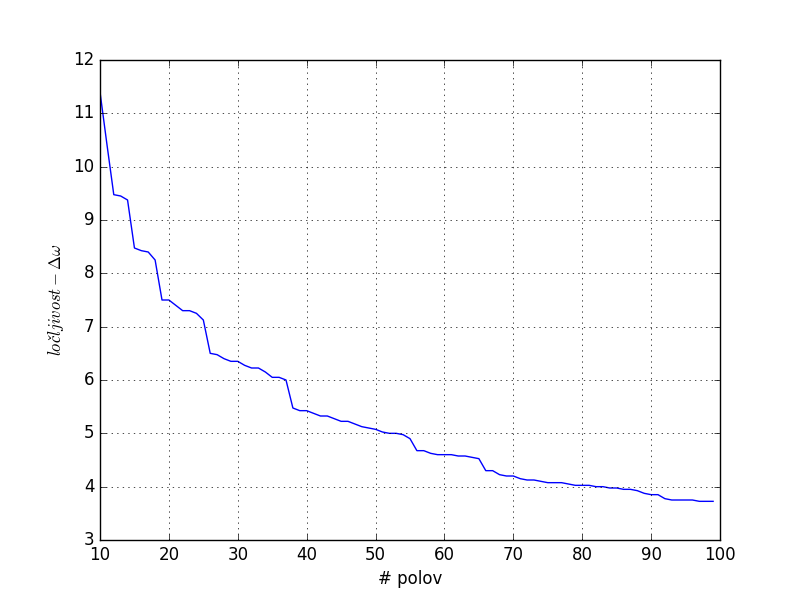
\includegraphics[scale=0.4]{slike/locljivost_mem_stevilo_polov.png}
%\caption{second figure}
\caption{Ločljivost metode MEM. Natančnost metode narašča približno eksponentno z naraščanjem števila koeficientov. Od ''oka'' se pri okoli $20$ koeficientih ločljivost zadovoljivo ustali, da v nadaljevanju uporabljamo $20$ koeficientov. }
\end{figure}






\subsection{Frekvenčni spekter iz datoteke \textsl{va2.dat} in \textsl{val3.dat}}

Oglejmo si kako ta metoda deluje na podatkih iz datotek \textsl{va2.dat} in \textsl{val3.dat}.





\begin{figure}[!htb]
\centering
\begin{minipage}{0.5\textwidth}
\centering
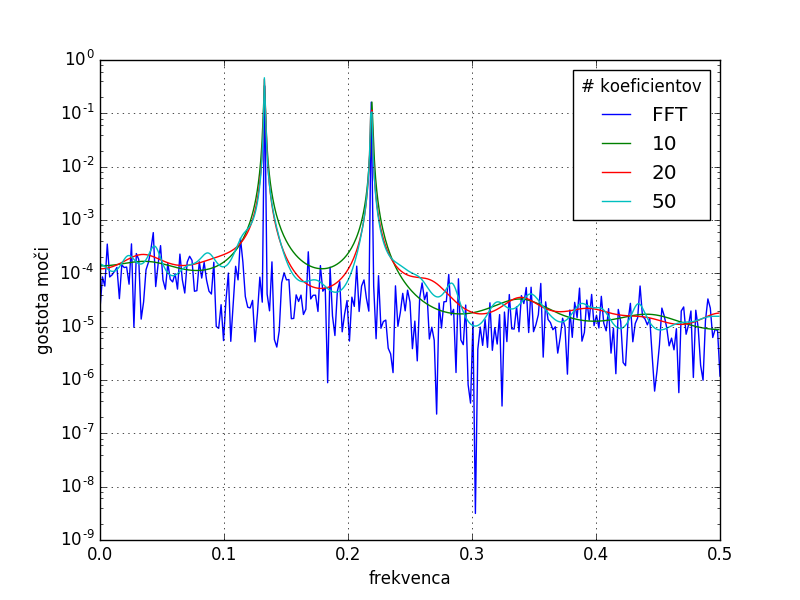
\includegraphics[scale=0.45]{slike/val2_primerjava_fft.png}
%\caption{first figure}
\end{minipage}\hfill
\begin{minipage}{0.5\textwidth}
\centering
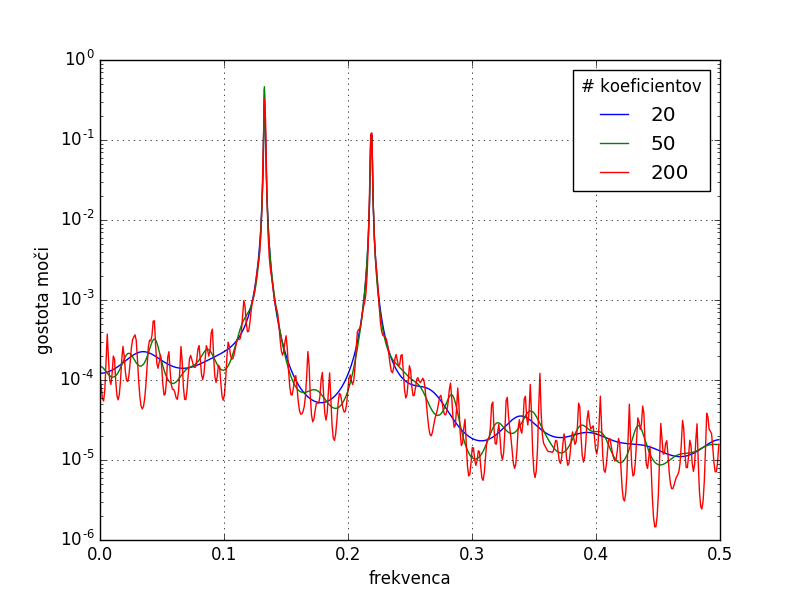
\includegraphics[scale=0.45]{slike/val2_primerjava_koef.png}
%\caption{second figure}
\end{minipage}

\caption{Primerjava spektrov podatkov iz datoteke \textsl{va2.dat}. Na levi imamo primerjavo MEM metode proti Fourierovi transformaciji (FT). Vidimo da je MEM metoda nekoliko zglajena FT, kar lahko sklepamo da dobro odtrani šum. Na desnem grafu vidimo, da z povečevanjem števila koeficientov ne izboljšamo odstranjevanja šuma, saj želi potem MEM metoda upoštevati tudi šum. }
\end{figure}



\begin{figure}[!hbt]
\centering
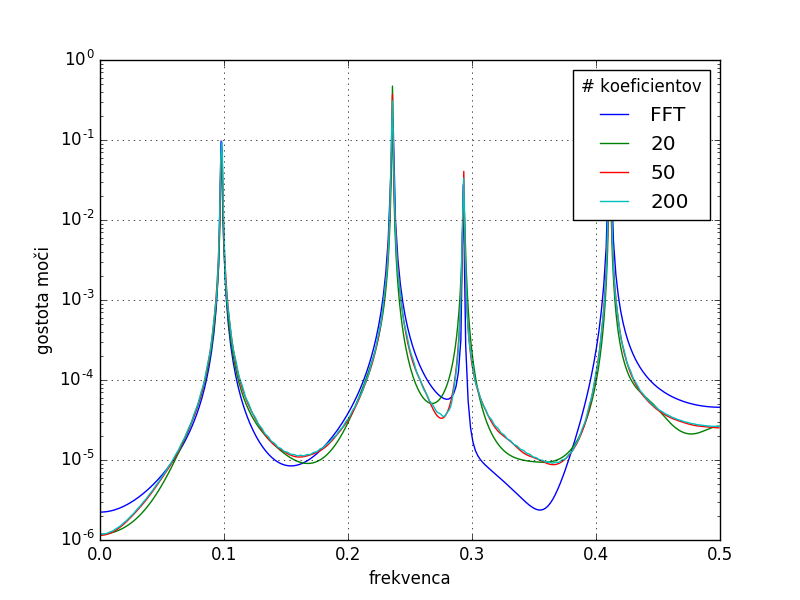
\includegraphics[scale=0.5]{slike/val3_primerjava_koef.png}
%\caption{second figure}
\caption{Frekvenčna slika iz datoteke \textsl{va3.dat}. V tem primeru sta MEM metoda in FT primerljivi. Obe metodi enako ostro določita vrhove. V tem primeru se z večanjem števila koeficientov ne izboljša spektralna oblika.}
\end{figure}

\FloatBarrier

\subsection{Koncentracija $CO_2$}

Imamo tudi meritve koncentracije $CO_2$ v zraku za preteklih $50$ let.
\begin{figure}[!htb]
\label{slika-co2}
\centering
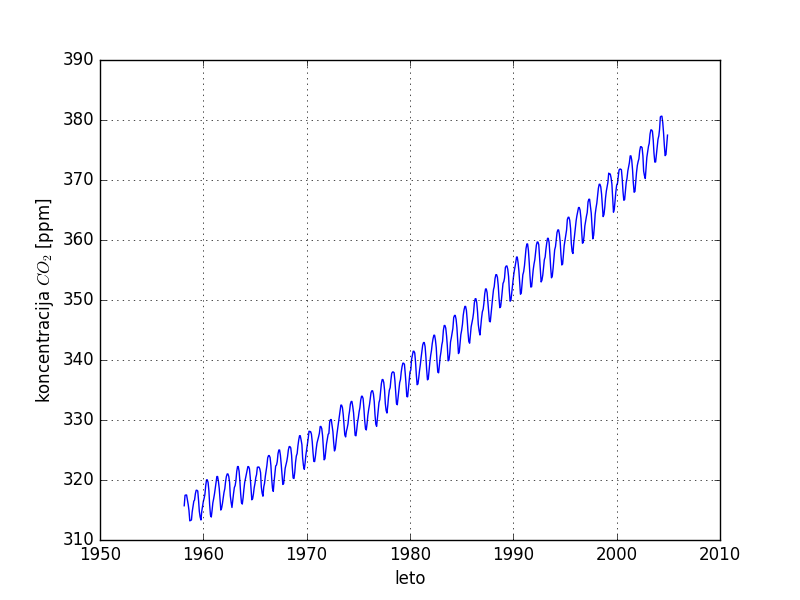
\includegraphics[scale=0.5]{slike/co2_koncentracija.png}
%\caption{second figure}
\caption{Koncentracija $CO_2$ v zraku skozi čas.}
\end{figure}
Nas zanima le frekvenčni oz. oscilirajoči del, zato bomo meritvam odšteli linearni člen.

\begin{figure}[!htb]
\label{slika-co2}
\centering
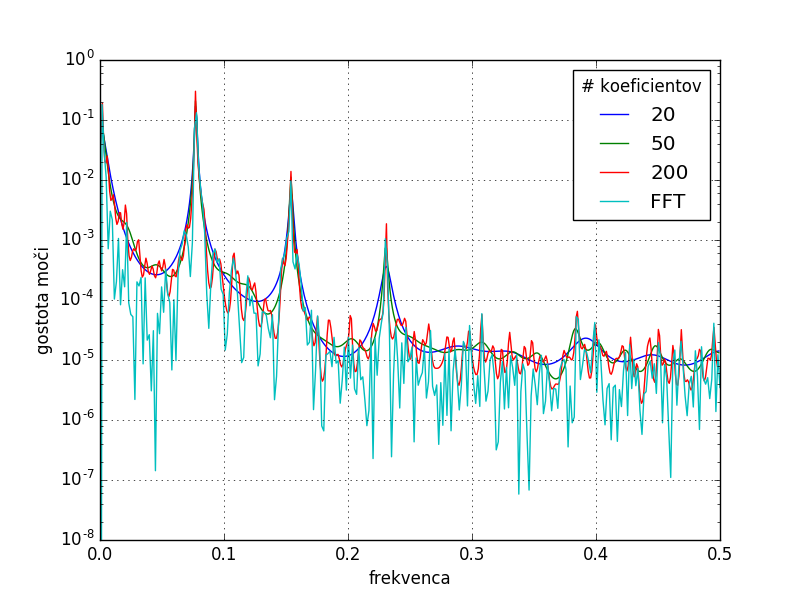
\includegraphics[scale=0.5]{slike/co2_primerjava_koef.png}
%\caption{second figure}
\caption{Frekvenčna slika meritev koncentracije $CO_2$ v ozračju. Iz slike opazimo nekaj izrazitih vrhov, kar nam očitno že graf \ref{slika-co2} pokaže. Ponovno se vidi, da z povečanjem števila koeficientov ne izboljšamo slike.}
\end{figure}






\begin{figure}[!h]
\centering
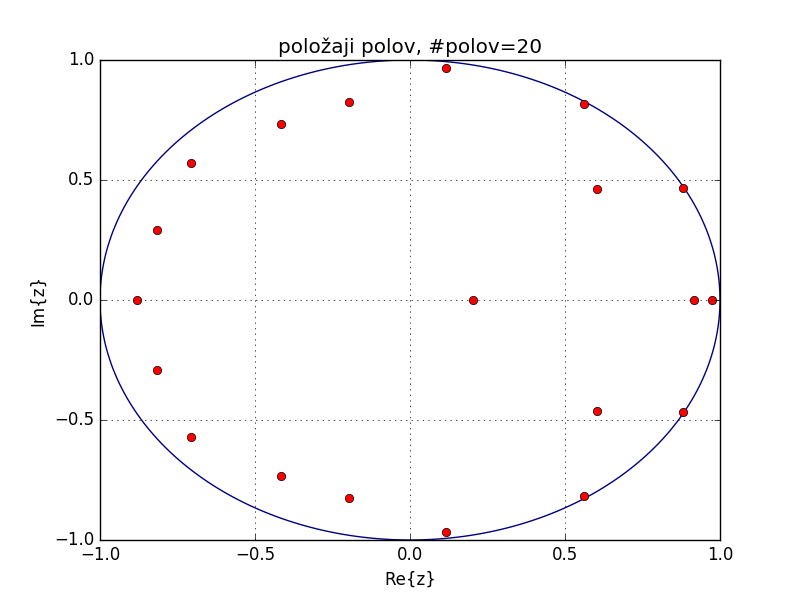
\includegraphics[scale=0.5]{slike/polozaji_polov.png}
%\caption{second figure}
\caption{Položaji polov pri MEM metodi za podatke meritev koncentracije $CO_2$. V tem primeru so vsi poli ležali izven enotske krožnice in so bili ustrezno transformirani znotraj krožnice. Uporabili smo $20$ polov.}
\end{figure}



\FloatBarrier

\section{Napoved}

Metodo maksimalne entropije smo začeli z trditvijo:

\begin{equation}
y_i=\sum_{k=1}^{N} a_k y_{i-k}
\end{equation}
kjer je trenutna vrednost meritve vsota predhodnih merjenih točk. Če torej že poznamo pretekle merjene točke in koeficiente $a_k$ lahko napovemo vrednost trenutne točke. To je poceni način za izračun vrednosti prihajajočih točk, saj izvajamo samo množenje in seštevanja.


\begin{figure}[!h]
\centering
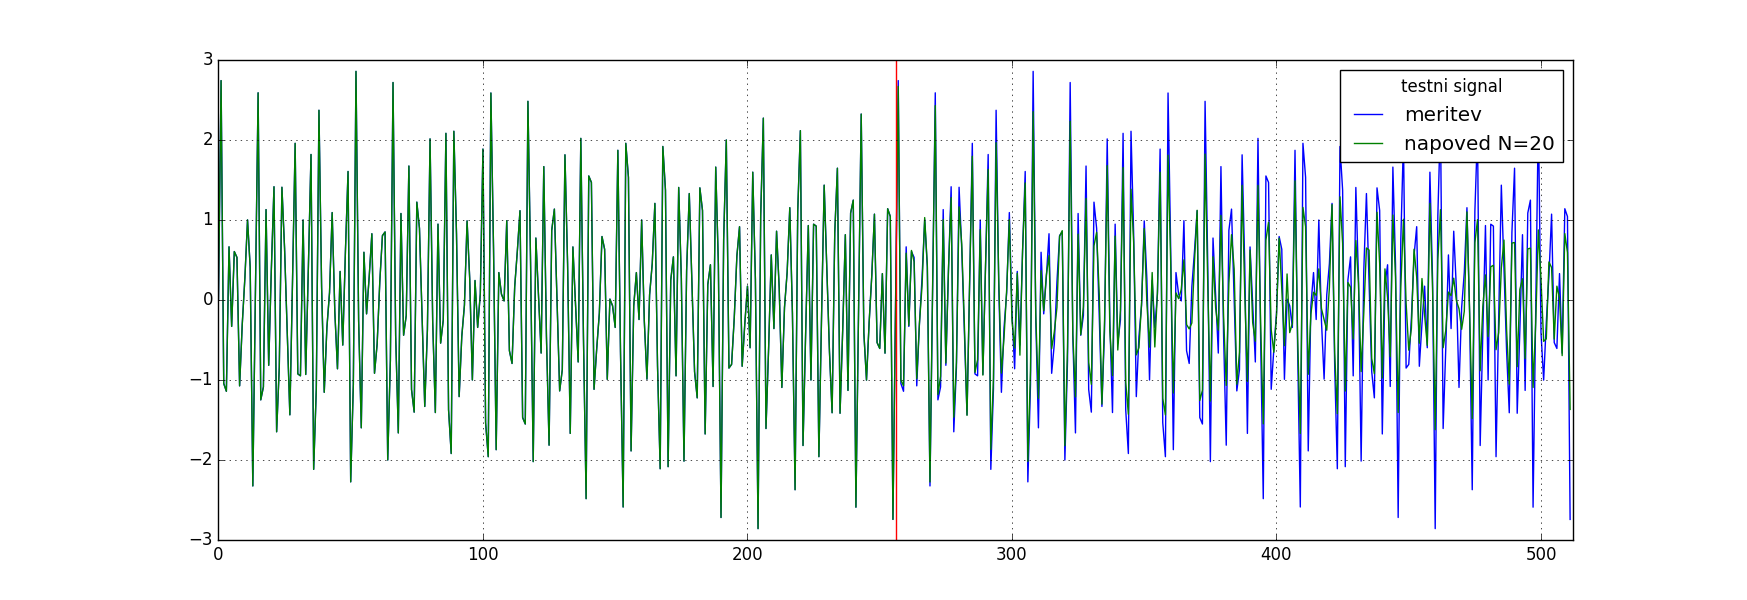
\includegraphics[scale=0.4]{slike/napoved_testni_sin2.png}
%\caption{second figure}
\caption{Napoved testnega signala iz prve naloge: $y_k= \sin(75 x_k) + \sin( 85 x_k)$. Opazimo, da je frekvenca oz. položaj vrhov sovpada z izmerjenimi vrednosti. Edina razlika je v velikosti vrhov, ki pa je različna. Verjetno je tu podoben vpliv, kot pri gostotni funkciji, kjer smo imeli dva različno velika vrhova. Rdeča navpična črta napoveduje začetek napovedi točk.}
\end{figure}




\begin{figure}[!h]
\centering
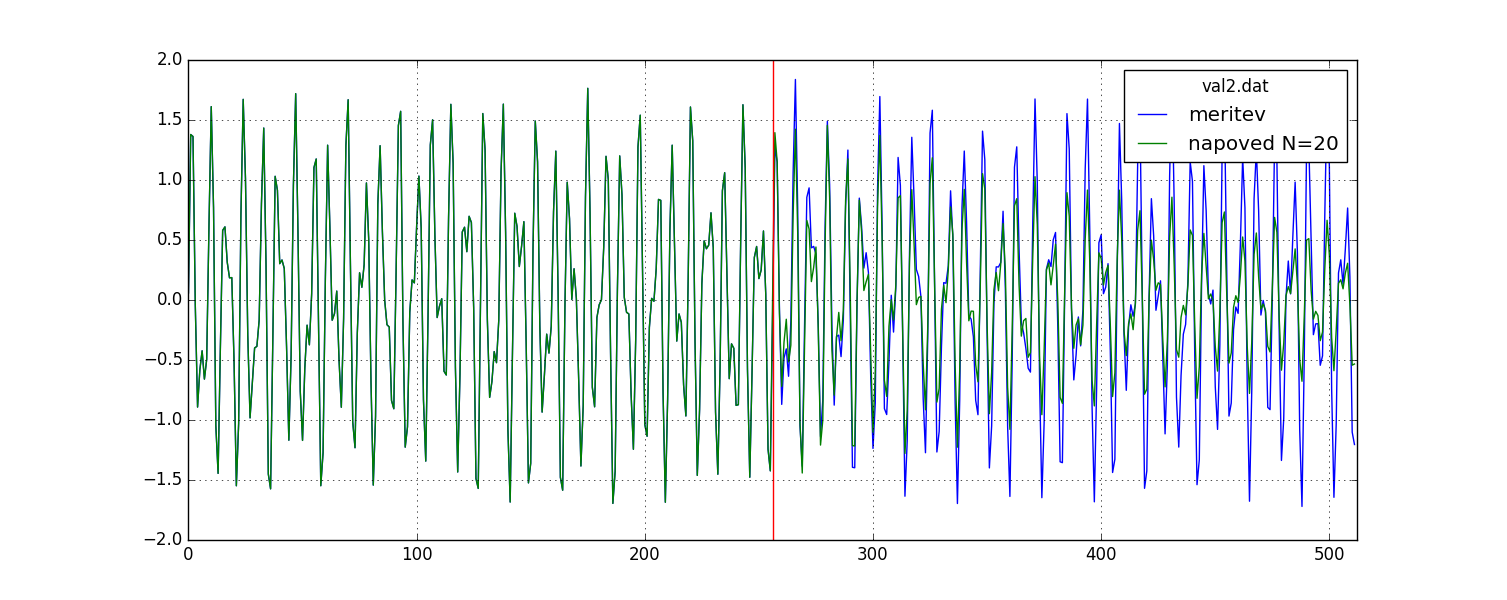
\includegraphics[scale=0.4]{slike/napoved_val2_2.png}
%\caption{second figure}
\caption{Napoved za podatke iz datoteke \textsl{val2.dat}.}
\end{figure}



\begin{figure}[!h]
\centering
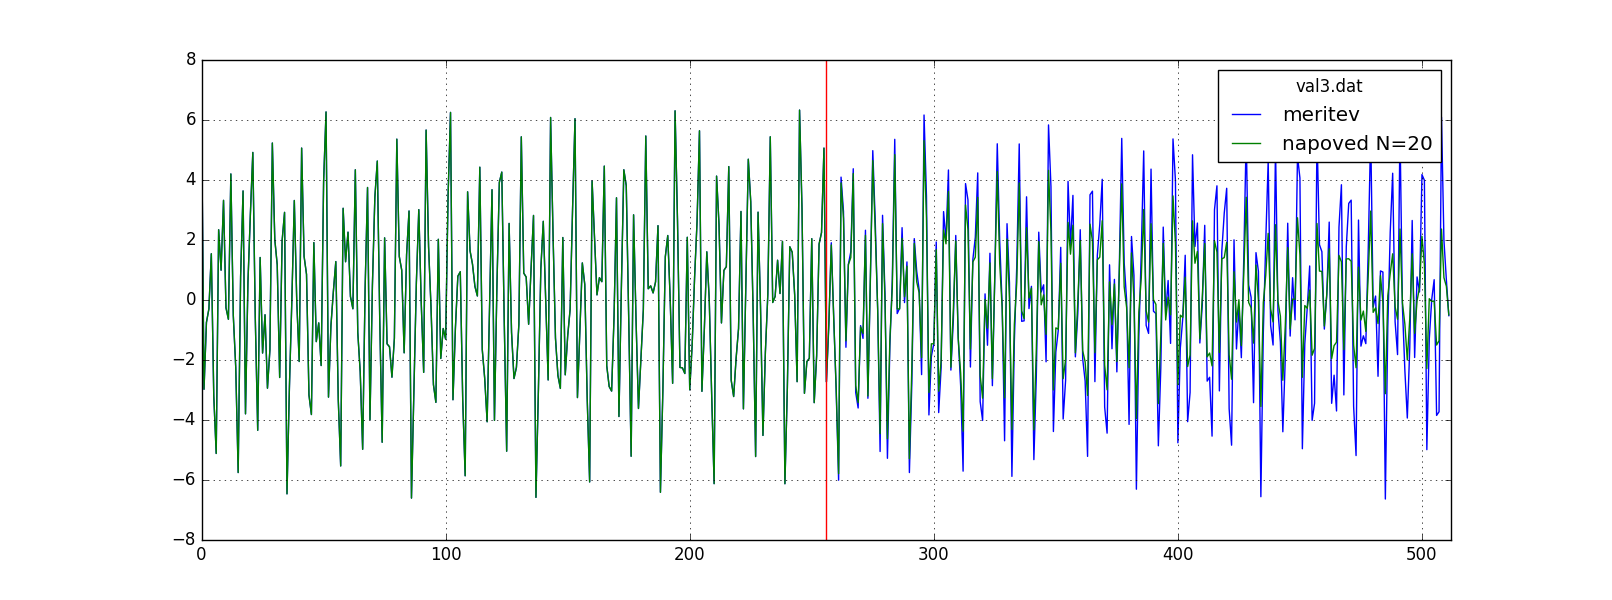
\includegraphics[scale=0.4]{slike/napoved_val3_2.png}
%\caption{second figure}
\caption{Napoved za podatke iz datoteke \textsl{val3.dat}.}
\end{figure}


\begin{figure}[!h]
\centering
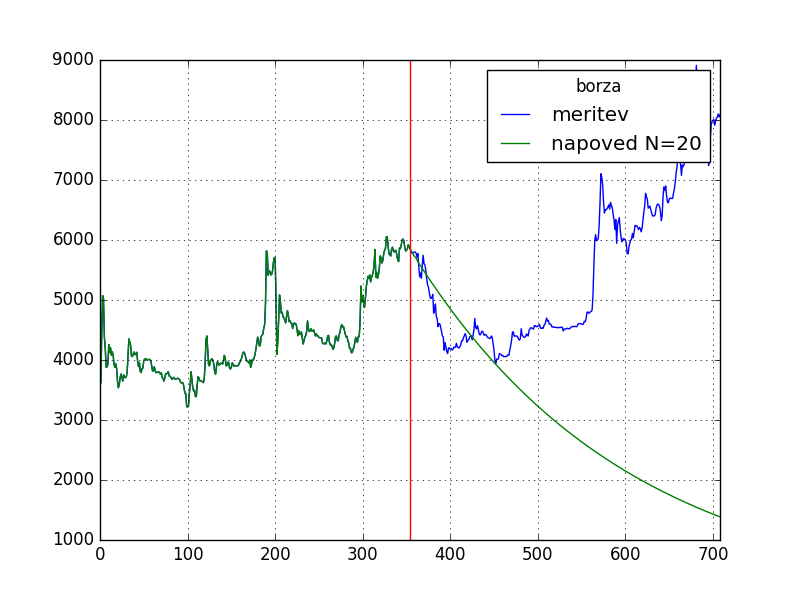
\includegraphics[scale=0.5]{slike/napoved_borza.png}
%\caption{second figure}
\caption{Napoved za podatke iz datoteke \textsl{borza.dat}.}
\end{figure}



\begin{figure}[!t]
\centering
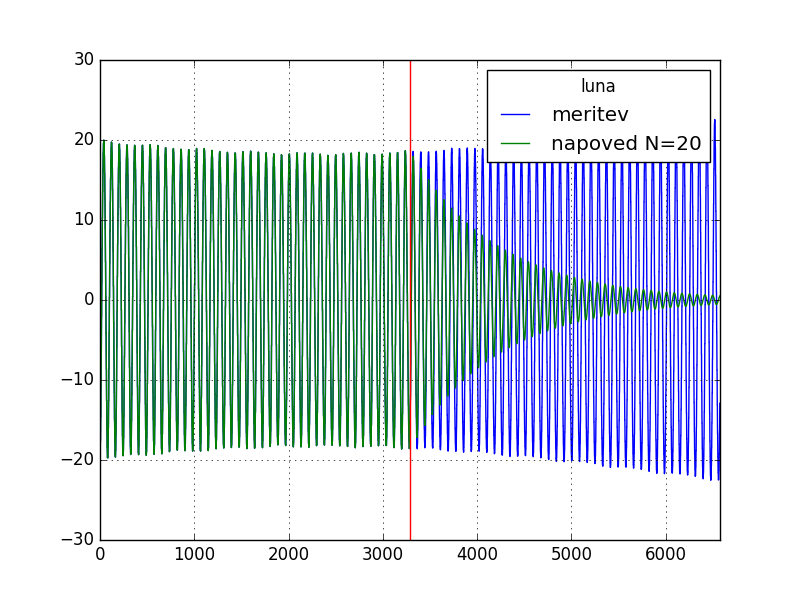
\includegraphics[scale=0.5]{slike/napoved_luna.png}
%\caption{second figure}
\caption{Napoved za podatke iz datoteke \textsl{luna.dat}.}
\end{figure}




\begin{figure}[!t]
\centering
\begin{minipage}{0.5\textwidth}
\centering
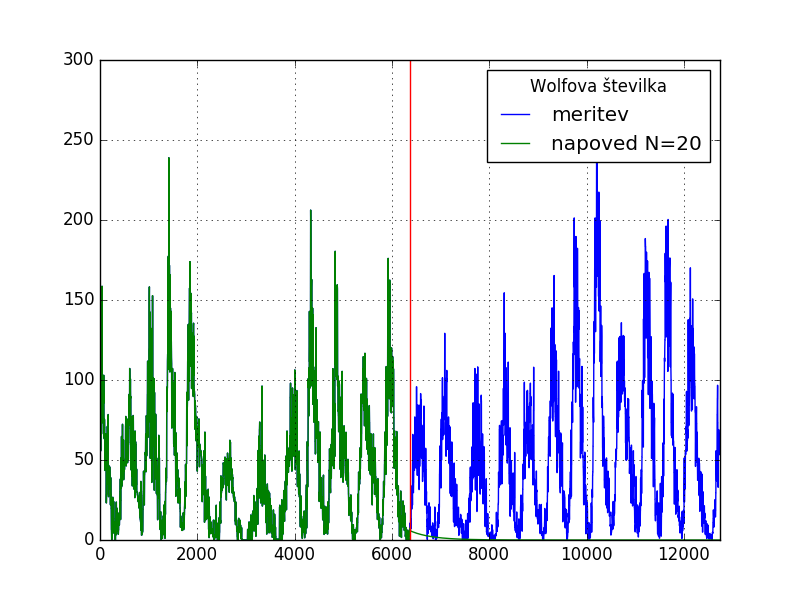
\includegraphics[scale=0.45]{slike/napoved_wolf20.png}
%\caption{first figure}
\end{minipage}\hfill
\begin{minipage}{0.5\textwidth}
\centering
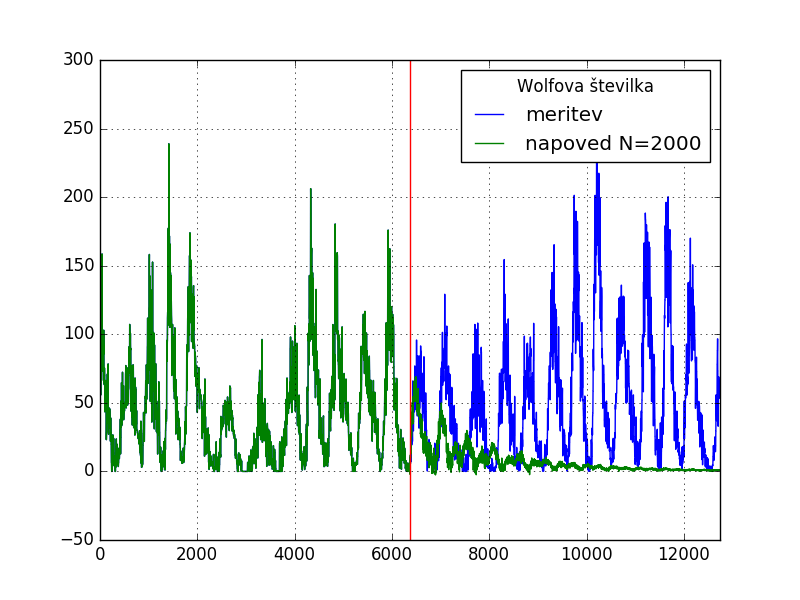
\includegraphics[scale=0.45]{slike/napoved_wolf2000.png}
%\caption{second figure}
\end{minipage}

\caption{Primerjava napovedi meritev iz datoteke \textsl{wolf.dat}. }
\end{figure}


\FloatBarrier

Če si ogledamo zgornje primere opazimo, da je ujemanje vrhov pri podatkih, ki so sestavljeni iz nekih periodičnih funkcij (npr. $\sin$ ali $\cos$). Pri napovedi \textsl{wolf.dat} je bilo potrebno za opazno periodično ujemanje povečati število koeficientov. Vzrok temu je najverjetneje majhna frekvenca, ki ima izrazit vrh v gostotni funkciji v primerjavi z vzorčno frekvenco in potrebujemo večje število koeficientov za opis sistema.\\
Pri ''nefrekvenčnih'' gibanjih (npr. borza), kjer podatki nakazujejo naključno gibanje ta metoda povsem odpove in lahko zaključimo, da je MEM metoda uporabna samo za določitev vrhov pri signalih sestavljeni iz periodičnih funkcij.

%---------------------------------------------------------------------------------------------------------


\end{document}
